\documentclass{beamer} % [handout] para imprimir eliminando transiciones

%\usefonttheme[onlymath]{serif}
%\usepackage{fontspec}
%\defaultfontfeatures{Mapping=tex-text}
%\setsansfont[Ligatures={Common}]{Futura}
%\setmonofont[Scale=0.8]{Monaco}

\usepackage{beamerthemesplit}
\usepackage[utf8]{inputenc}
\usepackage[spanish]{babel}
\mode<presentation>
\usetheme{default}
\usecolortheme{dolphin}
\usepackage{alltt}    % \begin{alltt}
\usepackage{amssymb}  % mathematical symbols
\usepackage{comment}
\usepackage{multicol} % \multicols
\usepackage{tabto}    % \tabto
\usepackage{verbatim} % comentarios

\title{Estructuras de datos}   %[titulo corto]
\author{Fabián Riquelme Csori} %[nombre corto]
\date{2017}                    %[fecha corta]
\institute{Universidad de Valparaíso}                 %[instituto corto]

\newcommand{\HRule}{\rule{\linewidth}{0.2mm}\\[1ex]}
\newcommand{\blue}[1]{\textcolor{blue}{#1}}
\newcommand{\red}[1]{\textcolor{red}{#1}}
\newcommand{\redb}[1]{{\color{red!70!black}{#1}}}
\newcommand{\green}[1]{{\color{green!70!black}{#1}}}
\newcommand{\gray}[1]{{\color{gray!50!white}{#1}}}
\newcommand{\textgreek}[1]{\begingroup\fontencoding{LGR}\selectfont#1\endgroup}
% \alert{texto destacado en rojo}
% \color{green} Color en verde
% \structure{texto en lila}

\begin{document}


%\begin{frame}%[plain]
%  \titlepage
%\end{frame}
%
% [opciones]:
% plain: oculta barra de navegacion, deja + espacio para contenido
% fragile: usar comandos como verbatim
% b,c,t: alineacion vertical
% label=nombre_etiqueta
% allowframebreaks: divide contenido en varios frames si es demasiado largo
% shrink: para escribir mucho texto en una transparencia, reduciendo tamano de fuente

%%%%%%%%%% PORTADA %%%%%%%%%%
\begin{frame}[plain]
  \begin{figure}[h]
    \begin{minipage}{0.3\textwidth}
    
\includegraphics[width=.9\textwidth]{./image/logo-UV.png}
    \end{minipage}
    \begin{minipage}{0.65\textwidth}
     $~$\\[3.6ex]
     \footnotesize{Escuela de Ingeniería Civil Informática}\\
     \footnotesize{Facultad de Ingeniería}
    \end{minipage}
  \end{figure}
  \begin{center}
    \vspace{1ex}
    \HRule
    \Large{Estructuras de datos}\\{\small Capítulo I: Análisis de algoritmos}\\[-1ex]
    \HRule\vspace{1ex}
    \large{Fabián Riquelme Csori}\\[.5ex]\footnotesize{fabian.riquelme@uv.cl}\\[6ex] {\tiny 2017-II}\\[6ex]
  \end{center}
\end{frame}

%%%%%%%%%% INDEX %%%%%%%%%%
\begin{frame}
 \frametitle{Index}
 \scriptsize 			% reducir tamano de letra
 \tableofcontents		%[pausesections]
\end{frame}

%%%%%%%%%%% ACTUAL INDEX %%%%%%%%%%
%\AtBeginSection[] %generar indice automaticamente
%{
%\begin{frame}<beamer>%[plain]
% \frametitle{Index}
% \framesubtitle{subtitulo}
% \scriptsize
% \tableofcontents[currentsection, currentsubsection]
%\end{frame}
%}

%==============================
\section{Tipos de datos}

%------------------------------
\subsection{Tipos de datos primitivos}

\begin{frame}{Tipos de datos}
    Un \blue{tipo de datos} es una propiedad o atributo de un conjunto de datos, que determina su dominio de aplicación, qué valores pueden tomar, qué operaciones se les pueden aplicar y cómo son representados internamente por el computador.
    \medskip\pause

    Un \blue{tipos de datos primitivo o elemental} es un tipo de datos proveído por un lenguaje de programación. Ejemplos:
    \pause

      \begin{multicols}{2}
      \begin{itemize}
        \item<3-> \texttt{char}
        \item<3-> \texttt{int}
        \item<3-> \texttt{float}
        \item<3-> \texttt{bool}
        \item<3-> \texttt{string}
        \item<3-> \texttt{pointer}
      \end{itemize}
      \end{multicols}
    \pause
    Estos tipos de datos primitivos se pueden mezclar para definir \blue{tipos de datos compuestos}. Por ejemplo, los \texttt{struct} en C y C++.
\end{frame}

%------------------------------
\subsection{Tipos de datos abstractos}

\begin{frame}{Tipos de datos abstractos}
    Un \blue{tipo de datos abstractos} (\blue{TDA}) es un modelo matemático para tipos de datos. Provee una descripción lógica o una especificación de los componentes del dato y de las \blue{operaciones} que son permitidas.
    \begin{itemize}
      \item<2-> Un TDA es indepediente de la implementación.
      \item<3-> Un TDA puede implementrse de diversas maneras incluso en un mismo lenguaje.
    \end{itemize}
    \uncover<4->{
    \begin{block}{Ventajas}
      \begin{multicols}{2}
      \begin{itemize}
        \item<5-> Encapsulamiento
        \item<5-> Localización de cambios
        \item<5-> Flexibilidad
        \item<5-> Reusabilidad
        \item<5-> Legibilidad
        \item<5-> ...
      \end{itemize}
      \end{multicols}
    \end{block}
    }
\end{frame}


\begin{frame}{Ejemplos de operaciones sobre TDA}
    \begin{itemize}
      \item<1-> \blue{Constructor} y \blue{destructor} (en POO)
      \item<2-> \blue{Iteradores}: para recorrer el dato.
      \item<3-> \blue{Operadores de capacidad}: determinar, verificar o modificar la capacidad de almacenamiento del dato.
      \item<4-> \blue{Operadores de acceso}: maneras de acceder a los elementos del dato.
      \item<5-> \blue{Modificadores}: maneras de modificar el contenido de los elementos del dato.
      \item<6-> \blue{Comparadores}: operadores (en general binarios) para relacionar datos del mismo TDA.
      \item<7-> Otros: swaps, replicadores, etc.
    \end{itemize}
    \uncover<8->{Ejemplo: \url{http://www.cplusplus.com/reference/vector/}}
\end{frame}

\begin{frame}{Eficiencia y complejidad}
    \begin{itemize}
      \item<1-> Se invierte mucho trabajo en mejorar la eficiencia de los TDA. De ello normalmente depende la eficiencia de todo el sistema.
      \item<2-> Pero ¿qué es la \blue{eficiencia}?
      \item<3-> Para medir tiempo de ejecución en bash desde  la shell de Linux, tenemos el comando \blue{\texttt{time}}:\\[1ex]
      \hspace{2ex} \texttt{real 0m0.037s}\\
      \hspace{2ex} \texttt{user 0m0.004s}\\
      \hspace{2ex} \texttt{sys 0m0.008s}\\
      \begin{itemize}
          \item<4-> \blue{\texttt{real}} es el tiempo total transcurrido para ejecutar la aplicación. Incluye otros procesos que estaban en ejecución.
          \item<5-> \blue{\texttt{user}} es el tiempo de CPU del proceso concreto que se ejecutó. Se excluye otros procesos y retardo de disco.
          \item<6-> \blue{\texttt{sys}} es el tiempo de CPU en llamadas al sistema del proceso.
          \item<7-> Si no hubieran otros procesos corriendo y la lectura de disco fuera inmediata, tendríamos \blue{\texttt{user}}$+$\blue{\texttt{sys}}$=$\blue{\texttt{real}}.
      \end{itemize}
    \end{itemize}
\end{frame}

\begin{frame}
   \begin{itemize}
      \item<1-> ¿Podemos hablar de eficiencia independientemente de los lenguajes de programación y de las máquinas?
      \item<2-> Complejidad temporal vs. complejidad espacial
      \begin{itemize}
          \item ¿Recuerdan las tablas de verdad de la lógica proposicional? ¿Conocen el problema SAT?
      \end{itemize}
    \end{itemize}
\end{frame}

%==============================
\section{Análisis de algoritmos}

%------------------------------
\subsection{Notación Big O}

\begin{frame}{Esfuerzo computacional}
  \begin{itemize}
    \item<1-> Dada una entrada \blue{$w$} para un algoritmo, definimos una función $T:\mathbb{N}\to\mathbb{N}$ tal que \blue{$T(|w|)$} es el tiempo o número de pasos que dicho algoritmo tarda en computar \blue{$w$}, en función de su tamaño \blue{$|w|$}.
    \item<2-> Dados dos algoritmos $A_1$ y $A_2$ que resuelven un mismo problema para una misma entrada $w$.\\ Sea $|w|=n$, supongamos:
    $$T_1(n)=n^3\mbox{ \, y \, }T_2(n)=6T_1(n)^2+3n+15$$
    \item<3-> Ambos algoritmos poseen un tiempo de ejecución \blue{polinomial}.
    \item<4-> No nos interesa tanto las diferencias ``sutiles'' entre $T_1$ y $T_2$, sino saber que ambos tiempos son polinomiales\\
    (i.e., nos concentramos en las \blue{tasas de crecimiento}).
  \end{itemize}
\end{frame}

\begin{frame}{Funciones superiormente acotadas: $O$}
  \begin{itemize}
      \item<1-> Todo polinomio está \blue{superiormente acotado} por otro polinomio.
      \item<2-> La tasa de crecimiento de cualquier polinomio puede representarse simplemente por su \blue{grado}.
      \item<3-> Ej: Si el \blue{tiempo de complejidad} de un algoritmo es $T(n)=3n^2+6n$, decimos que \blue{es del orden $n^2$}, y usamos la notación \blue{$O(n^2)$}, tal que \blue{$T(n)=O(n^2)$}.
      \item<4-> Formalmente,
      \redb{$$f(x)=O(g(x))$$}
      si existen $k,x_0$ reales positivos tal que
      $$|f(x)|\leq k\, |g(x)|\mbox{ , para todo } x\geq x_0$$
  \end{itemize}
\end{frame}

\begin{frame}{Algunas propiedades de Big O}
  \begin{block}{Adición}
    \begin{itemize}
      \item<1-> Si $f_1=O(g_1)$ y $f_2=O(g_2)$, entonces $f_1+f_2=O(|g_1|+|g_2|)$
      \item<2-> Si $f$ y $g$ son funciones positivas, $f+O(g)=O(f+g)$\\[2ex]
    \end{itemize}
  \end{block}
  \uncover<3->{
  \begin{block}{Multiplicación}
    \begin{itemize}
      \item<3-> Si $f_1=O(g_1)$ y $f_2=O(g_2)$, entonces $f_1f_2=O(g_1g_2)$
      \item<4-> $f\cdot O(g)=O(fg)$
      \item<5-> $O(kg)=O(g)$, para toda constante $k>0$.
    \end{itemize}
  \end{block}
  }
\end{frame}

\begin{frame}{Cotas usuales}
   \begin{itemize}
    \item \green{$O(1)$}        \tabto{14ex} es un crecimiento constante
    \item \green{$O(\log n)$}   \tabto{14ex} es un crecimiento logarítmico
    \item \green{$O(n)$}        \tabto{14ex} es un crecimiento lineal
    \item \green{$O(n^2)$}      \tabto{14ex} es un crecimiento cuadrático
    \item \green{$O(n^c)$}      \tabto{14ex} es un crecimiento polinomial
    \item \red{$O(c^n)$}, $c>1$ \tabto{14ex} es un crecimiento exponencial
    \item \red{$O(n!)$}         \tabto{14ex} es un crecimiento factorial
   \end{itemize}
\end{frame}

\begin{frame}{Algoritmos polinomiales vs. exponenciales}
  \begin{figure}[h]
    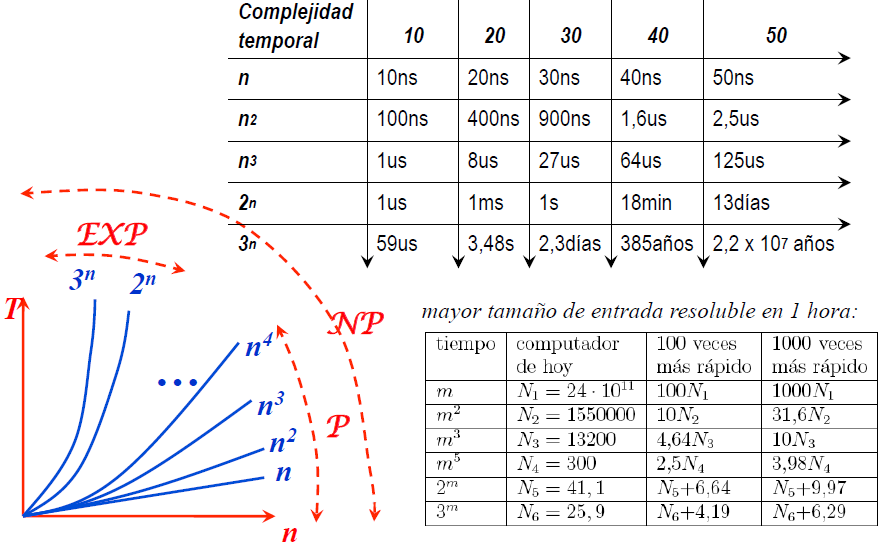
\includegraphics[width=\textwidth]{./image/cap1/EXP.png}
  \end{figure}
\end{frame}

\begin{frame}{Valorizando de forma General.}
  \begin{itemize}
    \item El análisis de programas sencillos se puede hacer contando los bucles anidados que contiene el programa. Un sólo bucle sobre n ítems genera f(n)=n. Un bucle dentro de otro bucle f( n ) = n2. Un bucle dentro de un bucle que está dentro de otro bucle genera f( n ) = n3.
    \item Dado un conjunto de bucles que son secuenciales, el más lento de ellos determina el comportamiento asintótico del programa. Dos bucles anidados, seguidos por un solo bucle, asintóticamente es lo mismo que los bucles anidados por sí solos, ya que los bucles anidados dominan el bucle individual.
    \end{itemize}
\end{frame}

\begin{frame}{Valorizando de forma General.}
  \begin{itemize}
    \item Regla General: Dado un conjunto de bucles que son secuenciales, el más lento de ellos determina el comportamiento asintótico del programa. Dos bucles anidados, seguidos por un solo bucle, asintóticamente es lo mismo que los bucles anidados por sí solos, ya que los bucles anidados dominan el bucle individual.
    \item Regla general: Programas con un Θ mayor corren más lentamente que programas con un Θ menor.
  \end{itemize}
\end{frame}

\begin{frame}{Valorizando de forma General.}
  \begin{itemize}
    \item Este filtro de eliminar todos los factores y de mantener el término de mayor crecimiento, como describimos anteriormente, es lo que denominamos asymptotic behavior. Entonces el comportamiento asintótico de f( n ) = 2n + 8 es descrito por la función f( n ) = n.
  \end{itemize}
\end{frame}

\begin{frame}
 \begin{block}{Bibliografía}
  \begin{itemize}
    \item Weiss, M., Estructura de datos y algoritmos,\\ Addison-Wesley, 1995.
    \item Aho, Hopcroft y Ullman, Estructuras de datos y algoritmos, Addison-Wesley, 1988.
  \end{itemize}
 \end{block}
 \begin{block}{Recursos}
  \begin{itemize}
    \item Wikipedia y Wikimedia Commons.
  \end{itemize}
 \end{block}
\end{frame}

\end{document}
